\documentclass[11pt,letterpaper,draft]{report}
\usepackage[left=3.5cm,right=3.5cm,top=2.5cm,bottom=2.5cm]{geometry}
\usepackage[english]{isodate}

\usepackage{amsmath,amsfonts,amsthm,bm,stmaryrd,amssymb}
\usepackage{enumitem,mathtools,multicol}
\usepackage[final]{graphicx}
%\pgfplotsset{compat=1.16}
\setenumerate[1]{label=\roman*).}
\setenumerate[0]{label=(\alph*)}
\allowdisplaybreaks

\newtheorem{exe}{Ejercicio}
\newtheorem{exa}{Ejemplo}
\newtheorem{lemma}{Lema}
\newtheorem{thm}{Teorema}
\newtheorem{rem}{Recordatorio}
\newtheorem{defn}{Definición}
\newtheorem*{sol}{Solución}

\newcommand\R{\mathbb R}
\newcommand\C{\mathbb C}
\newcommand\Z{\mathbb Z}
\newcommand\N{\mathbb N}
\newcommand\<{\langle}
\renewcommand\>{\rangle}
\let\cal\mathcal
\let\ol\overline
\DeclareMathOperator{\erf}{erf}
\DeclareMathOperator{\tr}{tr}
\DeclareMathOperator{\sgn}{sgn}
\DeclareMathOperator{\csch}{csch}
\title{Notas de clase}
\author{Jorge Alfredo Álvarez Contreras}

\begin{document}
\maketitle

\tableofcontents

\chapter{Sistemas lineales}

\subsection{Cálculo de $e^{At}$ para $A$ de $2\times 2$}

Sea $B=P^{-1}AP$, donde $P$ es la matríz formada por los vectores
característicos de $A$.
La matríz $B$ tiene una de las formas siguientes.

\begin{enumerate}
  \item
  $B=
  \begin{bmatrix}
    \lambda & 0 \\ 0 & \mu
  \end{bmatrix}
  $
  \item
  $B=
  \begin{bmatrix}
    \lambda & 1 \\ 0 & \lambda
  \end{bmatrix}$
  \item
  $B=
  \begin{bmatrix}
    a & -b \\ b & a
  \end{bmatrix}$
\end{enumerate}
Entonces, para cada caso, tenemos
\begin{enumerate}
  \item
  $e^{Bt}=
  \begin{bmatrix}
    e^{\lambda t} & 0 \\ 0 & e^{\mu t}
  \end{bmatrix}
  $
  \item
  $e^{Bt}=
  e^{\lambda t}
  \begin{bmatrix}
    1 & t \\ 0 & 1
  \end{bmatrix}$
  \item
  $e^{Bt}=
  e^{at}
  \begin{bmatrix}
    \cos bt & - \sin bt \\ \sin bt & \cos bt
  \end{bmatrix}$
\end{enumerate}
Así, $e^{At}=Pe^{Bt}P^{-1}$

\begin{exa}
  Resolver el sistema
  \[
    X' =
    \begin{bmatrix}
      -2 & -1 \\ 1 & -2
    \end{bmatrix}
    X,
    \hspace{10mm}
    X(0)
    =
    \begin{bmatrix}
      1 \\ 0
    \end{bmatrix}
  .\]
Obsérvese que $A$ es del tipo (iii) con $a=-2$ y $b=1$.
Entonces la solución es
\begin{align*}
  X(t)
  &= e^{At}x_0 \\
  &= e^{-2t}
  \begin{bmatrix}
    \cos t & -\sin t \\ \sin t & \cos t
  \end{bmatrix}
  \begin{bmatrix}
    1 \\ 0
  \end{bmatrix} \\
  &= e^{-2t}
  \begin{bmatrix}
    \cos t \\ \sin t
  \end{bmatrix} \\
  &= 
  \begin{bmatrix}
    e^{-2t}\cos t \\ e^{-2t}\sin t
  \end{bmatrix}
\end{align*}


Ahora $x_1^2+x_2^2=e^{-4t}$ o bien $|x(t)|=e^{-2t}$.
Esto es una espiral.

Si el valor inicial fuera $X(0)=(1,1)^T$, entonces
\begin{align*}
  X(t)
  &= e^{At}x_0 \\
  &= e^{-2t}
  \begin{bmatrix}
    \cos t & -\sin t \\ \sin t & \cos t
  \end{bmatrix}
  \begin{bmatrix}
    1 \\ 1
  \end{bmatrix} \\
  &= e^{-2t}
  \begin{bmatrix}
    \cos t - \sin t \\ \sin t + \cos t
  \end{bmatrix}
\end{align*}
\end{exa}

\begin{exa}
  \[
    X'=
    \begin{bmatrix}
      2 & -1 \\ 0 & 2
    \end{bmatrix}
    X,
    \hspace{10mm}
    X(0)=
    \begin{bmatrix}
      1 \\ 0
    \end{bmatrix}
  .\]

  Entonces $A$ es del topo (ii). Por lo tanto,
  \begin{align*}
    X(t)
    &= e^{2t}
    \begin{bmatrix}
      1 & -t \\ 0 & 1
    \end{bmatrix}
    \begin{bmatrix}
      1 \\ 0
    \end{bmatrix} \\
    &= e^{2t}
    \begin{bmatrix}
      1 \\ 0
    \end{bmatrix}
  \end{align*}
  
\end{exa}


\subsection{Sistema traza-determinante (2021 oct 28)}

Otra forma de determinar si el sistema $X'=AX$ tiene un nodo,
silla, espiral (foco) o centro en el punto $(0,0)$ es mediante el
sistema traza-determinante.

Si
\[
  A=
  \begin{bmatrix}
    a & b \\ c & d
  \end{bmatrix}
.\]
entonces $\tau=\tr A=a+d$ y $\Delta=\det A=ad-bc$.

\begin{enumerate}
  \item
  Si $\Delta<0$, entonces el sistema tiene un punto silla en el
  origen.
  
  \item
  Si $\Delta>0$ y $\tau^2-4\Delta>0$, entonces el sistema tiene
  un nodo. Es estable si $\tau<0$ e intestable si $\tau>0$.

  \item
  Si $\Delta>0$ y $\tau^2-4\Delta<0$ con $\tau\neq 0$, entonces
  el sistema tiene un espiral. Es estable si $\tau<0$ e inestable
  si $\tau>0$.

  \item
  Si $\Delta>0$ y $\tau^2-4\Delta<0$ con $\tau=0$, entonces el
  sistema tiene un centro.

  \item
  Si $\tau^2=4\Delta$, entonces el sistema tiene un nodo
  degenerado. Es estable si $\lambda<0$ e inestable si
  $\lambda<0$ e inestable si $\lambda>0$.
\end{enumerate}

\chapter{Sistemas no lineales (jue 11 nov 2021)}

Estamos estudiando el sistema
\begin{equation}\label{eqn:NL}
  X' = F(X)
\end{equation}
o bien
\begin{align*}
  x' &= P(x,y) \\
  y' &= Q(x,y).
\end{align*}
\begin{defn}[Punto crítico estable]
  Sea $X_1$ un punto crítico de \eqref{eqn:NL} y supóngase que
  $X=X(t)$ es la solución de \eqref{eqn:NL} que satisface
  $X(0)=X_0$ con $X_0\neq X_1$.
  Se dice que $X_1$ es estable cuando, dado un radio $\rho>0$
  existe un radio correspondiente $r>0$ tal que, si la posición
  inicial $X_0$ satisface
  \[
    |X_1\neq X_1|<r
  ,\]
  entonces $X(t)$ satisface $|X(t)-X_1|<\rho$ para todo $t>0$.

  Si, además, $\lim_{t\to\infty}X(t)=X_1$ para cualquier solución
  $X=X(t)$ con $|X(0)-X_1|<r$, decimos que $X_1$ es
  asintóticamente estable.
\end{defn}

\begin{exa}
  Considérese el sistema
  \begin{align*}
    r'(t) &= 0.05\cdot r(3-r) \\
    \theta'(t) &= -1
  \end{align*}

  \emph{Solución}:
  Si $r=0$ o $r=3$, tenemos $r'=0$. El sistema no tiene puntos
  críticos, pues $\theta'\neq 0$.

  Separando las variables en la primera ecuación, tenemos
  \begin{align*}
    t
    &= \int dt \\
    &= \int \frac{20\,dr}{r(3-r)} \\
    &= 20\int \left(\frac{1}{3r}+\frac{1}{3(3-r)}\right)\,dr \\
    &= \frac{20}{3} (\ln r-\ln(3-r) - \ln c_1).
  \end{align*}
  Multiplicando por $3/20$ y exponenciando
  \begin{align*}
    c_1e^{3t/20} &= \frac{r}{3-r}
  \end{align*}
  Así, $(3-r)c_1e^{3t/20}=r$, o bien
  $r+rc_1e^{3t/20}=3c_1e^{3t/20}$.
  Luego, la solución para $r(t)$ es
  \begin{align*}
    r(t)
    &= \frac{3c_1e^{3t/20}}{1+c_1e^{3t/20}} \\
    &= \frac{3c_1}{e^{-3t/20}+c_1}.
  \end{align*}
  Si $r(0)=r_0$, entonces $c_1=r_0/(3-r_0)$.
  Así,
  \begin{align*}
    r(t)
    &= \frac{3 \frac{r_0}{3-r_0}}{e^{-3t/20}+\frac{r_0}{3-r_0}}
    \\
    &= \frac{3r_0}{(3-r_0)e^{-3t/20}+r_0}.
  \end{align*}
  De aquí vemos que $r(t)\to 3$ conforme $t\to\infty$.
\end{exa}

\subsection{Linealización}
Rara vez es posible determinar la estabilidad de un punto crítico
del sistema $X'=F(X)$.
La idea de analizar la estabilidad es reemplazar la función
$F(X)$ por un término lineal de la forma $A(X-X_1)$, donde $X_1$
es un punto crítico del sistema que se aproxime a $F(X)$ cerca de
$X_1$.

En el caso de una variable
\[
  x' = g(x)
.\]
si $x_1$ es un punto crítico (es decir, $g(x_1)=0$), entonces $g$
tiene linealización alrededor de $x_1$ dada como
\begin{align*}
  Dg(x_1)(x-x_1)
  &= g(x_1) + g'(x_1)(x-x_1) \\
  &= g'(x_1)(x-x_1).
\end{align*}
Así, la linealización de la ecuación es
\[
  x' = g'(x_1)(x-x_1)
,\]
la cual es de variables separables.
Separando las variables, tenemos
\[
  \frac{dx}{x-x_1} = g'(x_1)\,dt
.\]
Es decir,
\[
  x-x_1 = c_1e^{g'(x_1)t}
,\]
o bien
\[
  x(t) = x_1+c_1e^{g'(x_1)t}
.\]
Así, si $g'(x_1)<0$, tenemos que $x(t)\to x_1$ conforme
$t\to\infty$. Es decir, en este caso, $x_1$ es asintóticamente
estable.
En caso de que $g'(x_1)>0$, entonces $x_1$ es asintóticamente
inestable.

\begin{exa}
  Consideremos la ecuación
  \[
    \frac{dx}{dt} = \cos x - \sin x
  .\]
  
  Aquí, $g(x)=\cos x-\sin x$.
  Entonces, considerando el intervalo $x\in(0,2\pi)$, tenemos que
  $g(x)=0$ si, y solo si, $x=\frac{\pi}{4}$ o $x=\frac{5\pi}{4}$.

  Tenemos que $g'(x)=-\sin x-\cos x$, por lo cual
  \begin{align*}
    g'(\tfrac{\pi}{4})
    &=-\sin \frac{\pi}{4}-\cos \frac{\pi}{4}
    =-\sqrt 2
    < 0,
    \\
    g'(\tfrac{5\pi}{4})
    &=-\sin \tfrac{\pi}{4}-\cos \frac{\pi}{4}
    =\sqrt 2
    > 0.
  \end{align*}
  Así, $\frac{\pi}{4}$ es un punto crítico asintóticamente
  estable y $\frac{5\pi}{4}$ es asintóticamente inestable.
\end{exa}

Para una función de dos variables, $z=g(x,y)$, la ecuación del
plano tangente en $(x_1,y_1)$ es
\[
  z = g(x_1,y_1) + \frac{\partial g}{\partial x}(x_1,y_1)(x-x_1)
  + \frac{\partial g}{\partial y}(x_1,y_1)(y-y_1)
.\]
Así, si $z_1=g(x_1,y_1)=0$, tenemos
\[
  z =
  \frac{\partial g}{\partial x}(x_1,y_1)(x-x_1)
  + \frac{\partial g}{\partial y}(x_1,y_1)(y-y_1)
.\]
Por lo tanto, si $X_1=(x_1,y_1)$ es un punto crítico del sistema
\begin{align*}\label{eqn:NL2}
  x' &= P(x,y) \\
  y' &= Q(x,y) \tag{1}
\end{align*}
entonces la linealización de este sistema cerca de $X_1$ es
\begin{align*}
  x' &= \frac{\partial P}{\partial x}(x_1,y_1)(x-x_1)
  + \frac{\partial P}{\partial y}(x_1,y_1)(y-y_1) \\
  y' &= \frac{\partial Q}{\partial x}(x_1,y_1)(x-x_1)
  + \frac{\partial Q}{\partial y}(x_1,y_1)(y-y_1).
\end{align*}
Es decir, el sistema $X'=F(X)$ se puede aproximar en la cercanía
de un punto crítico $X_1$ como
\begin{equation}\label{eqn:linealizacion}
  X' = JF(X_1)(X-X_1)
\end{equation}
donde $JF(X_1)$ es la matríz Jacobiana de $F=(P,Q)$ evaluada en
$X_1=(x_1,y_1)$:
\[
  JF(X_1)
  =
  \begin{bmatrix}
    \frac{\partial P}{\partial x} & \frac{\partial P}{\partial y}
    \\[2mm]
    \frac{\partial Q}{\partial x} & \frac{\partial Q}{\partial y}
  \end{bmatrix}_{(x_1,y_1).}
\]
Si en \eqref{eqn:linealizacion} se hace $H=X-X_1$, entonces
$H'=X'$, por lo cual obtenemos el sistema
\[
  H'=AH
\]
donde $A=JF(X_1)$.

\begin{thm}[Criterio de estabilidad]
  Sea $X_1$ un punto crítico del sistema \eqref{eqn:NL2}, donde
  $P$ y $Q$ tienen primeras derivadas parciales cercanadas a
  $X_1$.
  Entonces
  \begin{enumerate}
    \item Si los valores propios de $A$ tienen parte real
    negativa, entonces $X_1$ es asintótica\-mente estable.
    \item Si \emph{uno} de los valores propios de $A$ tiene parte
    real positiva, entonces $X_1$ es inestable.
  \end{enumerate}
\end{thm}

\begin{exe}
  Analizar la estabilidad de los puntos críticos de los sistemas
  \begin{enumerate}
    \item
    \begin{align*}
      x' &= x^2+y^2-6 \\
      y' &= x^2-y
    \end{align*}
    
    \item
    \begin{align*}
      x' &= \frac{x}{100}(100-x-y) \\
      y' &= \frac{y}{20}(60-y-x/5)
    \end{align*}
  \end{enumerate}
\end{exe}

\chapter{Modelos físicos}

\section{Péndulo no lineal (jue 2 dic 2021)}


\begin{center}
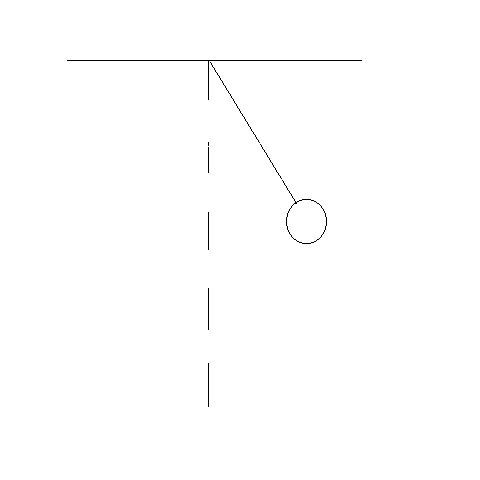
\includegraphics[width=0.5\textwidth]{img/pendulo-no-lineal}
\end{center}

Consideremos una barra de longitud $\ell$ a la cual se le coloca una
masa $m$. Suponiendo que no existen fuerzas externas ni de
amortiguamiento, se dice que el movimiento es libre.
Se desea determinar la ecuación que describa el movimiento de la masa
sobre la barra o el desplazamiento del ángulo $\theta$. Se considera
positivo si el desplazamiento es hacia la drecha, y negativo si es
hacia la izquierda.

Ahora, el arco $s$ de segmento del círculo de radio $l$ está dado por
$s=\ell\theta$.
Luego, la aceleración angular es
\[
  a=\frac{d^{2}s}{dt^{2}} = \ell \frac{d^{2}\theta}{dt^{2}}
.\]
Por la segunda ley de Newton $F=ma$, se tiene que
\[
  F=m\ell\frac{d^{2}\theta}{dt^{2}}
.\]
De acuerdo a la figura, la fuerza tangencial es $F=-mg\sin\theta$.
Igualando, tenemos
\[
  m\ell\frac{d^{2}\theta}{dt^{2}} = -mg\sin\theta
.\]
o bien
\[
  \boxed{
  \frac{d^{2}\theta}{dt^{2}} = -\frac{g}{l}\sin\theta
  .}
\]
Esta es una ecuación de segundo orden no lineal.
Tomando $x=\theta$, el sistema equivalente es
\begin{align*}
  x' &= y \\
  y' &= -\frac{g}{l}\sin x.
\end{align*}
Los puntos críticos son $(n\pi,0)$, donde $n\in\Z$.

Para el caso en que exista una amortiguación, esta es una fuerza de la
forma $bl\frac{d\theta}{dt}$, donde $b$ es la llamada constante de
fricción.
En este caso, la ecuación diferencial es
\[
  m\ell\frac{d^{2}\theta}{dt^{2}} =
  -mg\sin\theta-b\ell\frac{d\theta}{dt}
\]
o bien
\[
  \frac{d^{2}\theta}{dt}+\frac{b}{m}\frac{d\theta}{dt}
  +\frac{g}{l}\sin\theta = 0
.\]
Sea $\alpha=\frac{g}{l}$ y $\beta=\frac{b}{m}$. Entonces la ecuación
es
\[
  \boxed{
    \frac{d^{2}\theta}{dt}+\beta\frac{d\theta}{dt}
    +\alpha\sin\theta = 0
  .}
\]
Tomando $x=\theta$, el sistema equivalente es
\begin{align*}
  x' &= y \\
  y' &= -\alpha\sin x-\beta y.
\end{align*}

cuyos puntos críticos son $(n\pi,0)$ con $n\in\Z$.
Analizaremos el punto crítico $(0,0)$.

Dado que el fenómeno es un sistema físico, se sugiere usar como
función de Lyapunov a la suma de la energía cinética y la energía
potencial. Es decir,
\begin{align*}
  E_c &= \frac{1}{2}y^{2} \\
  E_p &= \int_{0}^{x}\alpha\sin u\,du \\
      &= -\alpha\cos u \Big|_{0}^{x} \\
      &= \alpha(1-\cos x),
  E(x,y) &= E_c+E_p \\
         &= \frac{\beta}{2}y^{2} + \alpha(1-\cos x).
\end{align*}
Esta función es definida positiva para $-\pi<x<\pi$.
Ahora la derivada es
\begin{align*}
  E'(x,y)
  &= \frac{dE}{dt} \\
  &= \alpha\sin x \cdot y - y(\alpha\sin x+\beta y) \\
  &= -\beta y^{2}
  &\leq 0.
\end{align*}
Por lo tanto, podemos asegurar que $(0,0)$ es estable. Sin embargo, no
se descarta que pueda ser asintóticamente estable.

Ahora, para $(\pi,0)$ con sideremos el cambio de variable $u=x-\pi$.
Entonces el sistema trasladado es
\begin{align*}
  x' &= y \\
  y' &= \alpha\sin(x-\pi) - \beta y.
\end{align*}
La energía total es
\[
  E = \frac{1}{2}y^{2} - \alpha(1+\cos(x-\pi))
\]
la cual no es definida positiva. No nos dice nada al respecto del
sistema.

\section{Cuenta deslizante}
Supóngase que una cuenta de masa $m$ se desliza a lo largo de un
alambre delgado cuya curva está dada por la función $z=f(x)$. La
fuerza tangencial $F$ debida al peso $w$ es $F=mg\sin\theta$ y la
componente en $x$ es $F_x=-mg\sin\theta\cos\theta$. Así,
\[
  F_x = -mg \frac{\sin\theta}{\cos\theta}\cos^{2}\theta
  =mg\tan\theta \frac{1}{\sec^{2}\theta}
.\]

Ahora, dado que $f'(x)=\tan\theta$, entonces
$\sec^{2}\theta=1+\tan^{2}\theta$.
Por lo tanto,
\[
  F_x = -mg\frac{f'(x)}{1+(f'(x))^{2}}
.\]
Ahora supongamos que existe una fuernza amortiguadora que se opone al
movimiento de la cuenta dada como $\beta\frac{dx}{dt}$. Si no existen
fuerzas externas, entonces por la segunda ley de Newton $F=ma$ se
tiene
\[
  m\frac{d^{2}x}{dt^{2}} = -mg\frac{f'(x)}{1+(f'(x))^{2}}
  -\beta\frac{dx}{dt}
\]
o bien
\[
  \frac{d^{2}x}{dt^{2}} = -g\frac{f'(x)}{1+(f'(x))^{2}}
  - \frac{\beta}{m} \frac{dx}{dt}
.\]
El sistema equivalente es
\begin{align*}
  x' &= y \\
  y' &= -g\frac{f'(x)}{1+(f'(x))^{2}}-\frac{\beta}{m}y.
\end{align*}
Sea $(x_1,y_1)$ un punto crítico del sistema. Entonces $y_1=0$,
por lo cual $f'(x_1)=0$, es decir:
el alambre es horizontal en ese punto.

La matríz jacobiana del sistema es
\[
  A
  =
  \begin{bmatrix}
    0 & 1 \\
    -g\frac{f''(x)(1-f'(x)^{2})}{(1+f'(x)^{2})^{2}}
      & -\frac{\beta}{m}
  \end{bmatrix} \Big|_{(x,y)=(x_1,y_1)}
  =
  \begin{bmatrix}
    0 & 1 \\
    -gf''(x_1) & -\frac{\beta}{m}
  \end{bmatrix}.
\]
Tenemos
\begin{align*}
  \tau &= -\frac{\beta}{m} \\
  \Delta &= gf''(x_1) \\
  \tau^{2}-4\Delta &= \frac{\beta^{2}}{m^{2}}-4gf''(x_1).
\end{align*}


\paragraph{Conclusión}

\begin{itemize}
  \item
    Si $f''(x)>0$ y $\beta\neq 0$,
    entonces el punto crítico $(x_1,0)$ es
    \begin{itemize}
      \item
        un nodo estable si $\beta^{2}>4m^{2}gf''(x_1)$,
      \item
        una espiral estable si $\beta^{2}<4m^{2}gf''(x_1)$
      \item
        un nodo degenerado estable si $\beta^{2}=4m^{2}gf''(x)$.
    \end{itemize}
  \item
    Si $f''(x_1)>0$ y $\beta=0$, entonces $(x_1,0)$ es un centro.
  \item
    Si $f''(x_1)<0$, entonces el punto $(x_1,0)$ es un punto silla.
\end{itemize}

\begin{exa}
  Considérese el caso de $f(x)=\sin x$, $m=0.01$, $g=9.81$ y
  $\beta^{2}=3.92\cdot 10^{-3}$.
  Entonces
\end{exa}


\end{document}
